\chapter{\approxtitle{Interval decomposition}}
\label{chap:betterapprox}

The $2k$-approximation
suffix-prefix decomposition algorithm
introduced in \cref{chap:2kapprox}
can be naturally improved
by spanning each of the $k$ intervals
of the given $k$-interval function
optimally using the minimization algorithm
introduced in \cref{chap:1interval}
(originally in \citet{Schieber2005154}).
We will call this improved algorithm
\quot{interval decomposition algorithm}.

Since the interval decomposition algorithm
clearly performs at least as well
as the suffix-prefix decomposition algorithm,
it is $2k$-approximation as well
(see \cref{theorem:spd2kapprox}).
\citeauthor{Dubovsky2012} has managed
to prove that on $2$-interval functions,
the interval decomposition algorithm
has an approximation ratio $2$
\citep[p.~39]{Dubovsky2012}, % Theorem 4.2
while the suffix-prefix decomposition algorithm
has a tight approximation ratio $4$
on $2$-interval functions
(see \cref{theorem:2kapproxtight}).
This might lead us to expect
that the interval decomposition algorithm
performs significantly better in general.
However,
we will show in this chapter that its approximation ratio
is close to $2k$ for large values of $k$.
\todomaybe{Add \quot{(and namely that it is strictly larger than $k$
for $k > 2$)} if we prove it.}

\section{\algdesctitle}

\todo[inline]{Label or name the algorithm properly and then refer to it consistently.}

\begin{algorithm}
[Interval decomposition]
\label{algorithm:id}

\hfill

\begin{description}
\item[Input]
\minintinput

\item[Output]
\minintoutput

\item[Procedure]
The algorithm spans each of the $k$ intervals
$\interval{a_i}{b_i}$ separately.
For every $i$,
let $\mathcal{T}_i$ be the spanning set of the interval
$\interval{a_i}{b_i}$ returned by the $1$-interval
optimization algorithm
introduced in \cref{chap:1interval}.
The algorithm returns
$\mathcal{T} = \bigcup_{i=1}^k{\mathcal{T}_i}$.
\end{description}
\end{algorithm}

Note that the spanning set constructed
by the interval decomposition algorithm
need not be disjoint
(unlike the spanning set constructed
by the suffix-prefix decomposition algorithm).
If we used \citeauthor{Schieber2005154}'s
$1$-interval disjoint spanning set minimization algorithm
\citep{Schieber2005154},
we would obtain a disjoint spanning set.
We will not analyze the approximation ratio in this case.
\todonote{We would need to find a good disjoint representation of the hard functions.}

\section{\titleapproxratio}

Let $F$ be a class of Boolean functions.
We shall denote the worst case approximation ratio
of the interval decomposition algorithm
on functions from class $F$ with $\approxid{F}$:
$$
\approxid{F}
= \sup_{f \in F}{\frac{id(f)}{dnf(f)}}
$$
\todo{Define properly with a label.}
\todo{Move to section 4 and simplify the description here.}
where $id(f)$ is the size of the spanning set of $f$
returned by the interval decomposition algorithm.

We will analyze the approximation ratio
of \cref{algorithm:id}
on the class of all $k$-interval Boolean functions for every $k$,
that is $\intervalfns{k}$
(see \cref{def:intervalfns}).
\todo{Move this discussion to \cref{chap:2kapprox}.}
We will not derive an exact approximation ratio of \cref{algorithm:id} on $\intervalfns{k}$,
instead we will show that $\approxidintk$ is upper bounded by $2k$ for a given number of intervals $k$ and we will provide a lower bound on the approximation ratio which for large $k$ converges to $2k$ as well.

\subsection{Upper bound of \texorpdfstring{$2k$}{2k}}

Since the interval decomposition algorithm
spans each of the $k$ intervals separately and optimally,
while the suffix-prefix decomposition algorithm
spans each of them separately and possibly non-optimally,
we get an upper bound $2k$
on $\approxidintk$ by \cref{theorem:2kapproxratio}:

\begin{observation}
\label{observation:approxidintkupper}
Let $k \geq 1$.
Then $\approxidintk \leq \approxspdintk = 2k$.
\todo{Define $\approxspdintk$.}
\end{observation}

However,
there are functions on which \cref{algorithm:id} performs strictly better than \cref{algorithm:spd}.
In fact, $\approxidintk$ is exactly $k$
for $k \in \curly{1, 2}$
as will be discussed in \cref{sec:approxidk12}.
Therefore the approximation ratio of $2k$ is not tight
in general.
In the rest of this chapter we shall show a lower bound on the approximation ratio which converges to $2k$ as $k$ increases to infinity.

\subsection{Known lower bounds for $k \in \curly{1, 2}$}
\label{sec:approxidk12}

\citeauthor{Dubovsky2012} has shown
that the approximation ratio is strictly smaller than $2k$
for $k = 2$,
as the algorithm is $2$-approximation
in this case \citep[p.~39]{Dubovsky2012}. % Theorem 4.2
Similarly,
it is obvious that the algorithm
gives an optimal result in case $k = 1$
(which corresponds to the approximation ratio $1$).
\begin{align}
\approxidint{1} &= 1 \\
\approxidint{2} &= 2
\end{align}

In the rest of this chapter
we shall construct a class of $k$-interval functions which show that the approximation ratio is strictly bigger than $k$ for $k$ as small as $3$.
\todokucera{tu trojku tam nějak zvlášť nezmiňujete, nebo jo?}
\todobartek{Trojku zmiňuji jako nejmenší počet intervalů, pro který je aproximační poměr větší než $k$, v \cref{example:approxidf24}.}
\todomaybe{Try to prove for all $k \geq 3$.}
We will even show that the approximation ratio of \cref{algorithm:id} is relatively close to $2k$ for large values of $k$.

\subsection{Difficult functions}
\label{sec:difficultfns}
\todokucera[inline]{a class of functions achieving the lower bound}

In this section we will describe a class of functions
on which the interval decomposition algorithm
performs particularly badly.
For every $l \geq 1$ and $n \geq l+2$,
we will construct
a proper $(2^{l-1} + 1)$-interval $n$-ary function $f_l^n$.

\begin{definition}
[Difficult function $f_l^n$]
\label{def:difficultfn}
%\label{def:difficultsuffix}
%\label{def:difficultprefix}

Let $l \geq 1$
denote a parameter that determines the number of intervals of $f_l^n$.
Let $n \geq l+2$
denote the arity of $f_l^n$
(and thus the length of its points,
especially the interval endpoints).
Let $k = 2^{l-1} + 1$ denote the number of intervals of $f_l^n$.

%Every interval endpoint
%$x \in \curly{a_1, b_1, \ldots, a_k, b_k}$
%has a prefix $p_x$ of length $l$
%and a suffix $s_x$ of length $n - l$.
%Note that $x = p_x s_x$.

The endpoints of the $k$ intervals
of the function $f^n_l$ shall be denoted as
$a_1, b_1, \ldots, a_k, b_k$,
that is the $i$-th interval of $f^n_l$
is $\interval{a_i}{b_i}$.
All the endpoints $a_1, \ldots, a_k$
have the same suffix $s_a = \rep{0}{n-l-1} 1$
and all the endpoints $b_1, \ldots, b_k$
have the same suffix $s_b = \rep{1}{n-l-1} 0$,
both of them having the length $n-l$.
\todonote[inline]{
Note that for $n \geq l + 3$,
this \quot{shape} corresponds to an extreme
non-trivial endpoint combination in the $1$-interval
optimization algorithm
(namely case \quot{$b' \geq a' - 1$}
in \cref{sec:1interval0011}),
which happens to be the case where the improvement
of the optimization algorithm
over the suffix-prefix approximation algorithm
is the largest.
}
Given an index $i \in \curly{1, \ldots, k}$
the endpoints $a_i$ and $b_i$ have the $l$-bit prefix
$p_{a_i}$ and $p_{b_i}$ which are defined as follows:
\begin{itemize}
\item $p_{a_1} = p_{b_1} = \rep{0}{l}$
% p_{a_2} = p_{b_1} + 1 = 1
% p_{b_2} = p_{a_2} + 1 = 2
% p_{a_3} = p_{b_2} + 1 = 3
% i p_{a_i}
% 1 0
% 2 1
% 3 3
% 4 5
% 5 7
\item $p_{a_i} = 2 \cdot i - 3$ for $i \in \curly{2, \ldots, k}$
% i=k: 2k-3 = 2^l + 2 - 3 = 2^l-1
% k=2^{l-1} + 1
\item $p_{b_i} = 2 \cdot i - 2$ for $i \in \curly{1, \ldots, k-1}$
\todomaybe{Remove duplicit definition of $p_{b_1}$ and $p_{a_k}$.}
\item $p_{a_k} = p_{b_k} = \rep{1}{l}$
\end{itemize}

To summarize our definition,
for a given index $i \in \curly{1, \ldots, k}$
we have that
$a_i = p_{a_i} s_a$ and $b_i = p_{b_i} s_b$.
We will prove that the function $f_l^n = \fnkab$
is a correctly defined proper $k$-interval function
in the observations that follow.
\end{definition}

\begin{example}
Let's consider the function $f_2^4$
(that is $f_l^n$ for $l=2$, $n=4$)
for example.
\cref{fig:f24} shows a schematic visualization
of this function.
The function $f_2^4$ consists of the three intervals
$\interval{0001}{0010}$, $\interval{0101}{1010}$
and $\interval{1101}{1110}$.

\begin{figure}[h]
\centering
% http://www.texample.net/tikz/examples/coin-flipping/
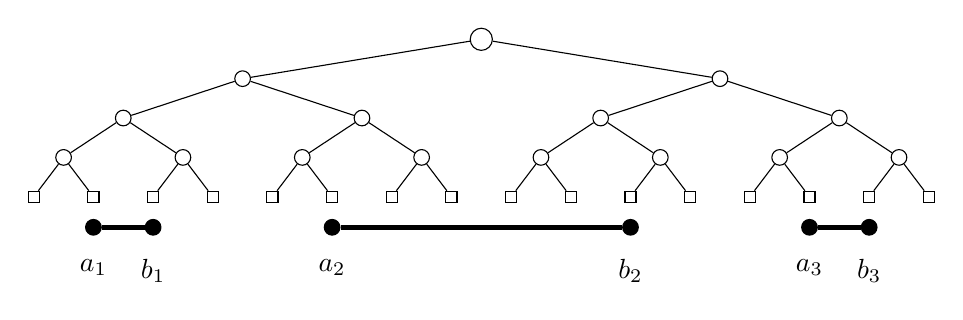
\begin{tikzpicture}[
    %scale = 1,
    %transform shape,
    %thick,
    %grow = down,  % alignment of characters
    level 1/.style = {sibling distance=\textwidth / 2},
    level 2/.style = {sibling distance=\textwidth / 4}, 
    level 3/.style = {sibling distance=\textwidth / 8}, 
    level 4/.style = {sibling distance=\textwidth / 16},
    level distance = 0.5cm,
    inner/.style = {draw, circle, inner sep=2pt},
    leaf/.style = {inner, rectangle},
    root/.style = {inner, minimum size=8pt},
    point/.style = {draw, circle, inner sep=2pt},
    truepoint/.style = {point, fill = black},
    falsepoint/.style = {point, fill = white},
    trueinterval/.style = {line width = 2pt}
  ]
  \node[root] (eps) {}
   child {   node[inner] (0) {}
     child { node[inner] (00) {}
       child { node[inner] (000) {}
         child { node[leaf] (0000) {}}
         child { node[leaf] (0001) {}}
       }
       child { node[inner] (001) {}
         child { node[leaf] (0010) {}}
         child { node[leaf] (0011) {}}
       }
     }
     child { node[inner] (01) {}
       child { node[inner] (010) {}
         child { node[leaf] (0100) {}}
         child { node[leaf] (0101) {}}
       }
       child { node[inner] (011) {}
         child { node[leaf] (0110) {}}
         child { node[leaf] (0111) {}}
       }
     }
   }
   child {   node[inner] (1) {}
     child { node[inner] (10) {}
       child { node[inner] (100) {}
         child { node[leaf] (1000) {}}
         child { node[leaf] (1001) {}}
       }
       child { node[inner] (101) {}
         child { node[leaf] (1010) {}}
         child { node[leaf] (1011) {}}
       }
     }
     child { node[inner] (11) {}
       child { node[inner] (110) {}
         child { node[leaf] (1100) {}}
         child { node[leaf] (1101) {}}
       }
       child { node[inner] (111) {}
         child { node[leaf] (1110) {}}
         child { node[leaf] (1111) {}}
       }
     }
   };

  % Labels
  \begin{scope}[nodes = {draw = none}]
    \begin{scope}[nodes = {below = 8pt}]
      \node [name = a1, truepoint] at (0001) {};
      \node [name = b1, truepoint] at (0010) {};
      \draw [trueinterval] (a1) -- (b1) node {};
      \node [name = a2, truepoint] at (0101) {};
      \node [name = b2, truepoint] at (1010) {};
      \draw [trueinterval] (a2) -- (b2) node {};
      \node [name = a3, truepoint] at (1101) {};
      \node [name = b3, truepoint] at (1110) {};
      \draw [trueinterval] (a3) -- (b3) node {};
    \end{scope}
    \begin{scope}[nodes= {below = 8pt}]
      \node at (a1) {$a_1$};
      \node at (b1) {$b_1$};
      \node at (a2) {$a_2$};
      \node at (b2) {$b_2$};
      \node at (a3) {$a_3$};
      \node at (b3) {$b_3$};
    \end{scope}
  \end{scope}
\end{tikzpicture}
\caption[A tree visualization of the function $f_2^4$]
{A tree visualization of the function $f_2^4$.
The leaves of the tree correspond to the $32$ $4$-bit binary vectors ordered from left to right in increasing order.
The three intervals of $f_2^4$ are shown below the tree.}
\label{fig:f24}
\end{figure}
\todokucera[inline]{Bylo by dobré v tom obrázku naznačit, kde končí prefix a začíná sufix (horizontální čárou, nebo tím, že spojnice v prefixu budou čárkovaně nebo pod.)}
\todo[inline]{Show again later with the optimal and ID spanning set.}
\end{example}

\todokucera[inline]{Ta [nálsedující; 2,3,4] tři pozorování bych dal do jednoho s odrážkami, před to bych napsal, „The following observation follows directly from the definition of the prefixes.“ Důkaz bych tam nedával, je to zřejmé, jako první odrážku by šlo třeba přidat, že $p_{b_1}=p_{a_1}$ a $p_{a_k}=p_{b_k}$, pokud to odstraníte z té definice.}

\begin{observation}
\label{observation:difficultaibi}
$p_{b_i} = p_{a_i} + 1$
for $i \in \curly{2, \ldots, k-1}$.
\end{observation}

\begin{proof}
The observation is a trivial application
of \cref{def:difficultfn}.
\end{proof}

\begin{observation}
\label{observation:difficultineqab}
$p_{a_i} \leq p_{b_i}$ for $i \in \curly{1, \ldots, k}$.
\end{observation}

\begin{proof}
The fact that
$p_{a_i} \leq p_{b_i}$ for $i \in \curly{2, \ldots, k-1}$
follows from \Cref{observation:difficultaibi}.
For $i \in \curly{1, k}$,
we have $p_{a_i} = p_{b_i}$
by \cref{def:difficultfn}.
\end{proof}

\begin{observation}
\label{observation:difficultprefixdist}
$p_{a_{i+1}} = p_{b_i} + 1$ for $i \in \curly{1, \ldots, k-1}$.
\end{observation}

\begin{proof}
We will show this by expanding \cref{def:difficultfn}
separately for various values of $i$.

\begin{itemize}
\item $i \in \curly{2, \ldots, k-2}$:

$p_{a_{i+1}}
= 2 \cdot (i+1) - 3
= 2 \cdot i - 1
= (2 \cdot i - 2) + 1
= p_{b_i} + 1$

\item $i = 1$:

$p_{a_2}
= 2 \cdot 2 - 3
= 1
= 0 + 1
= p_{b_1} + 1$

\item $i = k-1$:
\begin{align*}
p_{a_k}
&= \rep{1}{l} \\
&= 2^l - 1 \\
&= (2 \cdot 2^{l-1} - 2) + 1 \\
&= (2 \cdot ((2^{l-1} + 1) - 1) - 2) + 1 \\
&= (2 \cdot (k-1) - 2) + 1 \\
&= p_{b_{k-1}} + 1
\end{align*}
\end{itemize}
\end{proof}

\begin{corollary}
\label{corollary:difficultineqba}
$p_{b_i} < p_{a_{i+1}}$
for $i \in \curly{1, \ldots, k-1}$.
\end{corollary}

\begin{corollary}
\label{corollary:difficultineqbafull}
$b_i < a_{i+1}$
for $i \in \curly{1, \ldots, k-1}$.
\end{corollary}

\begin{observation}
\label{observation:difficultprefixlbit}
The numbers $p_{a_i}, p_{b_i}$
for $i \in \curly{1, \ldots, k}$
are correctly defined $l$-bit numbers.
\end{observation}

\begin{proof}
We need to show that none of the numbers $a_1, b_1, \ldots, a_k, b_k$
is smaller than $\rep{0}{l}$
or larger than $\rep{1}{l}$.

From \cref{observation:difficultineqab}
and \cref{corollary:difficultineqba}
it follows that $p_{a_1}$ is the smallest
and $p_{b_k}$ is the largest
of the numbers $p_{a_1}, p_{b_1}, \ldots, p_{a_k}, p_{b_k}$.
From \cref{def:difficultfn} we see that
$p_{a_1} = \rep{0}{l}$
and $p_{b_k} = \rep{1}{l}$.
\end{proof}

%Having shown both the $l$-bit prefix
%and the $(n-l)$-bit suffix of each endpoint,
%we are ready to make several observations
%that will come useful later.
%First let's check that the numbers
%$a_i = p_{a_i} s_{a_i}$
%and $b_i = p_{b_i} s_{b_i}$
%for $i \in \curly{1, \ldots, k}$
%actually are endpoints of a proper $k$-interval function
%by \cref{def:kibf,def:properkibf}.

\begin{observation}
\label{observation:difficultkintfn}
The numbers $a_1, b_1, \ldots, a_k, b_k$
are endpoints of a $k$-interval function
by \cref{def:kibf}.
\end{observation}

\begin{proof}
Clearly $a_1 \geq \rep{0}{n}$ and $b_k \leq \rep{1}{n}$,
since each of the numbers consists of an $l$-bit prefix
(see \cref{observation:difficultprefixlbit})
and an $(n-l)$-bit suffix
(see \cref{def:difficultfn}).

The fact that $a_i = p_{a_i} s_a \leq p_{b_i} s_b = b_i$
for $i \in \curly{1, \ldots, k}$ follows from
\cref{observation:difficultineqab}
and \cref{def:difficultfn}.

The fact that
$b_i < a_{i+1}$ for $i \in \curly{1, \ldots, k-1}$
follows from \cref{corollary:difficultineqbafull}.
\end{proof}

We conclude that $f_l^n$
is a correctly defined $k$-interval function.
We shall continue to show that $f_l^n$ is actually
a \emph{proper} $k$-interval function
by \cref{def:properkibf}.

\begin{observation}
\label{observation:difficultafp}
The vector $a_i - 1$ for $i \in \curly{1, \ldots, k}$
is a false point of $f_l^n$.
\end{observation}

\begin{proof}
First note that $a_i - 1 \geq 0$,
since $\bit{a_i}{n} = 1$ by \cref{def:difficultfn}.

Since $f_l^n$ is a correctly defined
$k$-interval function
by \cref{observation:difficultkintfn},
the vector $a_i - 1$
can only be a true point if
$i \geq 2$
and $a_i - 1 = b_{i-1}$.
However, this cannot happen because
$\bits{(a_i - 1)}{l+1}{n} = \rep{0}{n-l} \neq \rep{1}{n-l-1} 0 = \bits{b_{i-1}}{l+1}{n}$
by \cref{def:difficultfn}.
\end{proof}

\begin{corollary}
\label{corollary:difficultproper}
The function $f_l^n$
is a \emph{proper} $k$-interval function
by \cref{def:properkibf}.
\end{corollary}

We will continue to examine the properties of $f_l^n$
in several observations that will come useful later.

\begin{observation}
\label{observation:difficultprefixbeven}
$p_{b_i}$ is even
for every $i \in \curly{1, \ldots, k-1}$.
\end{observation}

\begin{proof}
This is easy to see from \cref{def:difficultfn}.
\end{proof}

\begin{observation}
\label{observation:difficultpreifxbevenequiv}
The numbers $p_{b_i}$ for $i \in \curly{1, \ldots, k-1}$
are exactly
all the $l$-bit even numbers.
\end{observation}

\begin{proof}
\hfill
\todokucera[inline]{Dohromady jste definoval k-1 po dvou různých sudých čísel, tedy $k-1=2^{l-1}+1-1=2^{l-1}$, víc sudých čísel do l bitů nenacpete, připadá mi to jako jednodušší argument, než rozbor níže.}
Every $p_{b_i}$ for $i \in \curly{1, \ldots, k-1}$
is $l$-bit by \cref{observation:difficultprefixlbit}
and it is even
by \cref{observation:difficultprefixbeven}.
%None of them is $\rep{0}{l}$,
%since $p_{b_1} = \rep{0}{l}$
%by \cref{def:difficultprefix}
%and $p_{b_{i+1}} \geq p_{a_{i+1}} > p_{b_i}$
%for $i \in \curly{1, \ldots, k-1}$
%by \cref{observation:difficultineqab,corollary:difficultineqba}.

To show that every $l$-bit even number
is equal to $p_{b_i}$
for some $i \in \curly{1, \ldots, k-1}$,
let $p_x$ be any $l$-bit even number
and let $i = \frac{p_x}{2} + 1$.
We claim that $i \in \curly{1, \ldots, k-1}$
and $p_x = p_{b_i}$.

\begin{enumerate}
\item $i \in \curly{1, \ldots, k-1}$:

It is easy to see that
if $p_x$ is even,
then $i$ defined as $\frac{p_x}{2} + 1$
is a whole number greater than or equal to $1$.
To see that $i \leq k-1$,
recall that $k = 2^{l-1} + 1$ by \cref{def:difficultfn}
and note that $p_x \leq \rep{1}{l-1} 0 = 2^l-2$
since $p_x$ is an $l$-bit even number.
The inequality follows:
\begin{align*}
i
&= \frac{p_x}{2} + 1 \\
&\leq \frac{2^l-2}{2} + 1 \\
&= 2^{l-1} - 1 + 1 \\
&= 2^{l-1} \\
&= k - 1
\end{align*}

\item $p_x = p_{b_i}$:
$$
p_{b_i}
= 2 \cdot i - 2
= 2 \cdot \round*{\frac{p_x}{2} + 1} - 2
= p_x + 2 - 2
= p_x
$$
\end{enumerate}
\end{proof}

\begin{observation}
\label{observation:difficultfpsuffix}
Every false point of $f_l^n$ ends with $\rep{0}{n-l}$
or $\rep{1}{n-l}$.
\end{observation}

\begin{proof}
Let $x$ be any $n$-bit binary vector.
Let $p_x = \bits{x}{1}{l}$ and $s_x = \bits{x}{l+1}{n}$.
We will prove the contrapositive
implication,
that is
if $s_x \notin \curly{\rep{0}{n-l}, \rep{1}{n-l}}$,
then $x$ is a true point.

It is easy to see that
$s_x \notin \curly{\rep{0}{n-l}, \rep{1}{n-l}}$
if and only if
$s_x \in \interval{\rep{0}{n-l-1} 1}{\rep{1}{n-l-1} 0}$, and that $x$ is a true point
if and only if
there is some $i \in \curly{1, \ldots, k}$
such that $x \in \interval{a_i}{b_i}$.
We will thus continue to prove the following statement
equivalent to \cref{observation:difficultfpsuffix}:
\begin{claim}
\label{claim:difficultfpsuffix}
Let
$s_x \in \interval{\rep{0}{n-l-1} 1}{\rep{1}{n-l-1} 0}$.
Let $i = \ceil{\frac{p_x}{2}} + 1$.
We claim that $i \in \curly{1, \ldots, k}$
and $x \in \interval{a_i}{b_i}$.
\end{claim}

\begin{itemize}
\item $i \in \curly{1, \ldots, k}$:

It is easy to see that $i$
defined as $\ceil{\frac{p_x}{2}} + 1$
is a whole number greater than or equal to $1$.
To see that $i \leq k$,
recall that $k = 2^{l-1} + 1$ by \cref{def:difficultfn}
and note that $p_x \leq 2^l-1$
since $p_x$ is an $l$-bit vector.
\begin{align*}
i &= \ceil*{\frac{p_x}{2}} + 1 \\
&\leq \ceil*{\frac{2^l-1}{2}} + 1 \\
&= \ceil*{2^{l-1} - \frac{1}{2}} + 1 \\
&= 2^{l-1} + 1 \\
&= k
\end{align*}

\item $x \in \interval{a_i}{b_i}$:

We will first show that $p_x \in \interval{p_{a_i}}{p_{b_i}}$.

To see that $p_{a_i} \leq p_x$:
\begin{align}
p_{a_i} \leq p_x
&\iff 2 \cdot i - 3 \leq p_x \\
&\iff 2 \cdot \round*{\ceil*{\frac{p_x}{2}} + 1} - 3 \leq p_x \\
&\iff 2 \cdot \ceil*{\frac{p_x}{2}} + 2 - 3 \leq p_x \\
&\iff 2 \cdot \ceil*{\frac{p_x}{2}} \leq p_x + 1
\label{ineq:difficultprefix}
\end{align}

It is easy to see that
the inequality \labelcref{ineq:difficultprefix} holds
in case $p_x$ is even.
In case $p_x = 2r + 1$ for some $r$:
\begin{align*}
2 \cdot \ceil*{\frac{p_x}{2}}
&= 2 \cdot \ceil*{\frac{2r + 1}{2}} \\
&= 2 \cdot \ceil*{r + \frac{1}{2}} \\
&= 2 \cdot \round*{r + \ceil*{\frac{1}{2}}} \\
&= 2 \cdot (r + 1) \\
&= 2r + 2 \\
&= (2r + 1) + 1 \\
&= p_x + 1
\end{align*}

We conclude that $p_{a_i} \leq p_x$.

To see that $p_{b_i} \geq p_x$:
\begin{align*}
p_{b_i}
&= 2 \cdot i - 2 \\
&= 2 \cdot \round*{\ceil*{\frac{p_x}{2}} + 1} - 2 \\
&= 2 \cdot \ceil*{\frac{p_x}{2}} + 2 - 2 \\
&= 2 \cdot \ceil*{\frac{p_x}{2}} \\
&\geq p_x
\end{align*}

Since $p_{a_i} \leq p_x$ and $s_a \leq s_x$
(by \cref{def:difficultfn}
$s_a = \rep{0}{n-l-1} 1$,
and by the premise of \cref{claim:difficultfpsuffix}
$s_x \geq \rep{0}{n-l-1} 1$),
$a_i = p_{a_i} s_a \leq p_x s_x = x$.
A symmetric argument shows that $b_i \geq x$.
\end{itemize}

We have shown that every point that does not end with
$\rep{0}{n-l}$ or $\rep{1}{n-l}$
is a true point of $f_l^n$.
Conversely
\todoforkucera{Is this word correct?}
every false point of $f_l^n$
ends with $\rep{0}{n-l}$ or $\rep{1}{n-l}$.
\end{proof}

\begin{observation}
\label{observation:difficulttpinb}
The true points of $f_l^n$
that end with $\rep{0}{n-l}$
are exactly all the points $p_{b_i} \rep{0}{n-l}$
for $i \in \curly{2, \ldots, k-1}$.
\end{observation}

\begin{proof}
Let $x$ be any $n$-bit binary vector.
Let $p_x = \bits{x}{1}{l}$
and $s_x = \bits{x}{l+1}{n} = \rep{0}{n-l}$.
We claim that $x$ is a true point of $f_l^n$
if and only if
$p_x = p_{b_i}$ for some $i \in \curly{2, \ldots, k-1}$.

\begin{enumerate}
\item If $f_l^n(x) = 1$,
then $p_x = p_{b_i}$
for some $i \in \curly{2, \ldots, k-1}$:

Let $x$ be a true point of $f_l^n$.
Let $\interval{a_i}{b_i}
= \interval{p_{a_i} s_a}{p_{b_i} s_b}$
be the interval of $f_l^n$ that contains $x$.
We claim that $i \in \curly{2, \ldots, k-1}$
and $p_x = p_{b_i}$.

\begin{enumerate}
\item $i \in \curly{2, \ldots, k-1}$:
\label{item:difficulttpi}

If $i \in \curly{1, k}$,
then $p_{a_i} = p_{b_i}$ by \cref{def:difficultfn}.
Since $s_a = \rep{0}{n-l-1} 1$
by \cref{def:difficultfn},
the interval $\interval{a_i}{b_i}$
does not contain any vector
that ends with $\rep{0}{n-l}$
and thus does not contain $x$ in particular.
Since $x$ is a true point,
necessarily $i \in \curly{2, \ldots, k-1}$.

\item $p_x = p_{b_i}$:

It is easy to see that
$p_x \in \interval{p_{a_i}}{p_{b_i}}$
(otherwise $x \notin \interval{a_i}{b_i}$).
Since $p_{b_i} = p_{a_i} + 1$
by \cref{item:difficulttpi,observation:difficultaibi},
$p_x$ is equal to either $p_{a_i}$ or $p_{b_i}$.
It cannot be $p_{a_i}$
since $p_{a_i} s_x
= p_{a_i} \rep{0}{n-l}
= p_{a_i} \rep{0}{n-l-1} 1 - 1
= a_i - 1$
is a false point
by \cref{observation:difficultafp},
so necessarily $p_x = p_{b_i}$.
\end{enumerate}

\item If $p_x = p_{b_i}$
for some $i \in \curly{2, \ldots, k-1}$,
then $f_l^n(x) = 1$:

Let $p_x = p_{b_i}$
for some $i \in \curly{2, \ldots, k-1}$
($x = p_{b_i} \rep{0}{n-l}$).
Since $p_{b_i} = p_{a_i} + 1$
by \cref{observation:difficultaibi},
$x \geq a_i$.
Since $s_x = \rep{0}{n-l}$ and $p_x = p_{b_i}$,
$x \leq b_i$.
We conclude that $x \in \interval{p_{a_i}}{p_{b_i}}$
and thus $f_l^n(x) = 1$.
\end{enumerate}

We conclude that the true points that end with $\rep{0}{n-l}$
are exactly the points $p_{b_i} \rep{0}{n-l}$
for $i \in \curly{2, \ldots, k-1}$.
\end{proof}

\subsection{Interval decomposition spanning set size}

Let $f_l^n =
f^n_{\interval{a_1}{b_1}, \ldots, \interval{a_k}{b_k}}$
be a $k$-interval function
defined in \cref{def:difficultfn}.
In this section we will express
\todokucera{[Before: show] evaluate? estimate?}
the size of the spanning set
returned by the interval decomposition algorithm
when run on this function.
We will denote its size with $id(f_l^n)$.

The interval decomposition algorithm spans
each of the intervals separately
using the optimization algorithm
from \cref{chap:1interval},
so $id(f_l^n) = \sum_{i=1}^k{\size{\mathcal{T}_i}}$,
where $\mathcal{T}_i$ is the spanning set
of the interval $\interval{a_i}{b_i}$
returned by the optimization algorithm
for $1$-interval functions.

For every $i$,
we shall analyze how the $1$-interval algorithm solves
the instance $\interval{a_i}{b_i}$.
We will divide the analysis between the intervals
for which $p_{b_i} = p_{a_i}$
(that is $i \in \curly{1, k}$)
and the ones for which $p_{b_i} = p_{a_i} + 1$
(that is $i \in \curly{2, \ldots, k-1}$;
see
\cref{def:difficultfn,observation:difficultaibi}).

\subsubsection{$i \in \curly{1, k}$}

In case $i \in \curly{1, k}$,
the endpoints have common prefixes of length $l$
($p_{b_i} = p_{a_i}$).
Thus the instance $\interval{a_i}{b_i}$
is reduced to the instance
$\interval{s_{a_i}}{s_{b_i}}
= \interval{\rep{0}{n-l-1} 1}{\rep{1}{n-l-1} 0}$.

Recall that $n \geq l + 2$ by \cref{def:difficultfn}.

If $n = l + 2$,
the instance
$\interval{\rep{0}{n-l-1} 1}{\rep{1}{n-l-1} 0}
= \interval{01}{10}$
is spanned using the procedure
shown in \cref{sec:1interval0110}.
This procedure spans the two trivial sub-intervals
$\interval{01}{01}$ and $\interval{10}{10}$
separately,
producing $2 = n-l$ ternary vectors.

If $n \geq l + 3$,
the instance
$\interval{\rep{0}{n-l-1} 1}{\rep{1}{n-l-1} 0}$
is spanned using the procedure
shown in \cref{sec:1interval0011}.
This procedure reduces the instance
to the instance $\interval{01}{10}$,
which again contributes $2$ ternary vectors,
and adds $n-l-2$ extra ternary vectors
that span the sub-interval
$\interval{\rep{0}{n-l-2} 10}{\rep{1}{n-l-2} 01}$.
The spanning set of the interval in this case has the size
$2 + n - l - 2 = n - l$.

We conclude that in case $i \in \curly{1, k}$,
$\size{\mathcal{T}_i} = n-l$.

\subsubsection{$i \in \curly{2, \ldots, k-1}$}

In case $i \in \curly{2, \ldots, k-1}$,
recall that $p_{b_i} = p_{a_i} + 1$
by \cref{observation:difficultaibi}.
This means that $p_{a_i} = c 0 \rep{1}{m}$
and $p_{b_i} = c 1 \rep{0}{m}$
for some binary vector $c$
and a number $m \in \curly{0, \ldots, l-1}$.

To see that $m \geq 1$,
recall that $p_{b_i}$ is even
by \cref{observation:difficultprefixbeven}.

This means that $a_i$ and $b_i$
start with a common prefix $c$
followed by the bits $01$ in $a_i$
and $10$ in $b_i$.
In the $1$-interval optimization algorithm,
the common prefix $c$ is left out
and then the procedure
shown in \cref{sec:1interval0110}
is applied to the remainder of the endpoints
(that is
$\interval{01 \rep{1}{m-1} s_{a_i}}
{10 \rep{0}{m-1} s_{b_i}}$).
This procedure spans the two sub-intervals
$\interval{\rep{1}{m} s_{a_i}}{\rep{1}{m+n-l}}$
and $\interval{\rep{0}{m+n-l}}{\rep{0}{m} s_{b_i}}$
separately using the suffix and prefix procedure
respectively
(see \cref{sec:prefixsuffix}).

Let's consider the sub-interval
$\interval{\rep{0}{m+n-l}}{\rep{0}{m} s_{b_i}}$;
the other one is symmetric.

Note that this sub-interval can be immediately reduced
to $\interval{\rep{0}{n-l}}{s_{b_i}}$
by removing the common prefix of the endpoints.

Recall that the prefix algorithm
produces one ternary vector
for each bit that is set to $1$
in $s_{b_i} + 1 = \rep{1}{n-l}$.
The returned spanning set of
$\interval{\rep{0}{n-l}}{s_{b_i}}$
thus has the size $n-l$.
Prepending the prefix $p_{b_i}$
we get a spanning set of
$\interval{p_{b_i} \rep{0}{n-l}}{p_{b_i} s_{b_i}}$.

We span the complementary sub-interval
$\interval{p_{a_i} s_{a_i}}{p_{a_i} \rep{1}{n-l}}$
in a symmetric manner,
getting another spanning set of size $n-l$.

Joining the sub-interval spanning sets together
we get the spanning set $\mathcal{T}_i$ of size $2(n-l)$.

\hfill

From the above considerations
we can conclude the following proposition:
\begin{lemma}
\label{lemma:difficultid}
$\mathit{id}(f_l^n) = 2^l(n-l)$
\end{lemma}

\begin{proof}
\begin{align*}
id(f_l^n) &= \sum_{i=1}^k{\size{\mathcal{T}_i}} \\
&= 2 (n-l) + \sum_{i=2}^{k-1}{2 (n-l)} \\
&= 2 (n-l) + (k-2) 2 (n-l) \\
%&= 2 (n-l) (1 + (k-2)) \\
&= 2 (n-l) (k-1) \\
&= 2 (n-l) ((2^{l-1} + 1) - 1) \\
%&= 2 (n-l) 2^{l-1} \\
&= 2^l (n-l)
\end{align*}
\end{proof}

\subsection{Minimum spanning set size}

In this section we will show a spanning set
of $f^n_l$ of size $n+l-2$
and prove its optimality
($dnf(f^n_l) = n+l-2$).

\begin{lemma}
\label{lemma:difficultdnfupper}
$dnf(f_l^n) \leq n+l-2$
\end{lemma}

\begin{proof}
We will show a spanning set $\mathcal{T}$
of $f_l^n$ of size $n+l-2$.
We will span the union of the intervals
$\interval{p \rep{0}{n-l-1} 1}{p \rep{1}{n-l-1} 0}$
for all $p \in \booldom^l$
using $n-l$ ternary vectors
and then we will add $2l-2$
vectors
to span the remaining true points.

First recall that by \cref{observation:difficultfpsuffix}
all the false points of $f_l^n$
end with either $\rep{0}{n-l}$ or $\rep{1}{n-l}$.
This means we need to span all the points that end
with different $(n-l)$-bit suffixes.
We can do that with the set $\mathcal{T}_{\mathit{out}}$
defined in the following way:
\begin{align*}
\mathcal{T}_{\mathit{out}}
&= \curly{\rep{\phi}{l} s
| s \text{ is a cyclic shift of } 01 \rep{\phi}{n-l-2}} \\
&= \curly{
\rep{\phi}{l} 01 \rep{\phi}{n-l-2},
\rep{\phi}{l} \phi 01 \rep{\phi}{n-l-3},
\ldots,
\rep{\phi}{l} 1 \rep{\phi}{n-l-2} 0
}
\end{align*}

To see that $\mathcal{T}_{\mathit{out}}$
spans all the points
that do not end with $\rep{0}{n-l}$ or $\rep{1}{n-l}$,
note that for every $(n-l)$-bit binary vector $x$
that contains both a $0$ and a $1$ as its component,
there is a position $i$
such that $\bit{x}{i} = 0$
and $\bit{x}{(i+1) \bmod (n-l)} = 1$.
Thus we have spanned the union of the intervals
$\interval{p \rep{0}{n-l-1} 1}{p \rep{1}{n-l-1} 0}$
for all $p \in \booldom^l$
using $n-l$ ternary vectors.

There are still some true points left for us to span,
namely those that end with $\rep{0}{n-l}$
or $\rep{1}{n-l}$.
Recall that by \cref{observation:difficulttpinb}
the true points that end with $\rep{0}{n-l}$
are exactly all the points $p_{b_i} \rep{0}{n-l}$
for $i \in \curly{2, \ldots, k-1}$.
Also recall that all such $p_{b_i}$ are even numbers
by \cref{observation:difficultprefixbeven}.
In fact,
$p_{b_i}$ for $i \in \curly{2, \ldots, k-1}$
are all the $l$-bit even numbers except $\rep{0}{l}$
(this is easy to see from
\cref{observation:difficultpreifxbevenequiv}
and the fact that $p_{b_1} = \rep{0}{l} < p_{b_2}$
\todomaybe{Reference observations.}).
We will employ the technique of cyclic shifts
again
to span these points efficiently.

Let $\mathcal{T}_0$ be the set defined as follows:
$$
\mathcal{T}_0 = \curly{c 0 \rep{0}{n-l}
| c \text{ is a cyclic shift of } 1 \rep{\phi}{l-2}}
$$

To see that $\mathcal{T}_0$ spans all the true points
that end with $\rep{0}{n-l}$,
note that the cyclic shifts of $1 \rep{\phi}{l-2}$
span exactly all the $(l-1)$-bit numbers
that contain a $1$
and the vectors $c 0$
where $c$ is a cyclic shift of $1 \rep{\phi}{l-2}$
span exactly all the $l$-bit \emph{even} numbers
that contain a $1$.
Clearly $\size{\mathcal{T}_0} = l-1$.

Symetrically we construct $\mathcal{T}_1$ of size $l-1$
that spans all the true points
that end with $\rep{1}{n-l}$.

Putting the partial spanning sets together,
we get the size of a spanning set of $f_l^n$:

\begin{align*}
\size{\mathcal{T}}
&= \size{\mathcal{T}_{\mathit{out}}}
+ \size{\mathcal{T}_0} + \size{\mathcal{T}_1} \\
&= (n-l) + (l-1) + (l-1) \\
&= n + l - 2
\end{align*}
\end{proof}

Having shown a spanning set of $f_l^n$ of size $n+l-2$,
we conclude that $dnf(f_l^n) \leq n+l-2$.

By further analysis we can even show that $dnf(f^n_l)=n+l-2$.
Although this fact is not needed to show the lower bound on the approximation ratio,
we include it here for completeness.

\begin{lemma}
$dnf(f_l^n) \geq n+l-2$
\end{lemma}

\todonote[inline]{We needn't prove this for the final result but it makes the following writing more legible.
It may be interesting to note, though, that the functions $f_l^n$ which are difficult to approximate are in fact coverable, and thus the difficulty in ID-approximation doesn't coincide with the difficulty in proving optimality of a spanning set (i.e. non-coverability), although both begin to be interesting for $k \geq 3$.}

\begin{proof}
We will show that $f_l^n$ can not be spanned
using fewer than $n+l-2$ ternary vectors
by showing an orthogonal set of $f_l^n$ of size $n+l-2$.
By \cref{theorem:orthodnf},
this proves that all the spanning sets of $f_l^n$
have the size at least $n-l-2$.

The orthogonal set $V$ consists of 3 components:
\begin{itemize}
\item
$V_{out} = \curly{\rep{0}{l} s
| s \text{ is a cyclic shift of } 1 \rep{0}{n-l-1}}$
\item
$V_0 = \curly{c 0 \rep{0}{n-l}
| c \text{ is a cyclic shift of } 1 \rep{0}{l-2}}$
\item
$V_1 = \curly{c 1 \rep{1}{n-l}
| c \text{ is a cyclic shift of } 0 \rep{1}{l-2}}$
\end{itemize}

To see that the sets $V_{out}$, $V_0$ and $V_1$
are pairwise disjoint,
consider any $v_{out} \in V_{out}$,
$v_0 \in V_0$ and $v_1 \in V_1$.
The vector $v_1$ differs from both $v_{out}$ and $v_0$
in the $l$-th position.
The vector $v_0$ differs from $v_{out}$
in the position $i \in \curly{1, \ldots, l-1}$
such that $\bit{v_0}{i} = 1$.

Since the sets $V_{out}$, $V_0$ and $V_1$
are pairwise disjoint,
their union $V$
has the size
$\size{V_{out}} + \size{V_0} + \size{V_1}
= (n-l) + (l-1) + (l-1) = n+l-2$.

For $V$ to meet the criteria of orthogonality
by \cref{def:orthogonal},
we need to show that every vector in $V$
is a true point of $f_l^n$
and that every pair of distinct vectors in $V$
is orthogonal.
\todomaybe{Rephrase -- inconsistent use of \quot{orthogonal}.}

\begin{claim}
$V \subseteq TP(f_l^n)$
\end{claim}

\begin{proof}

\hfill
\todo[inline]{Proof in a proof! Is this okay?}
\todokucera[inline]{Já osobně to rád nemám, ale někdo to používá. Mě připadá, že to ten důkaz pouze znepřehledňuje, na druhou stranu chápu, že v některých případech to má své opodstatnění, pokud se vám to tady líbí, tak proč ne.
Co kdybyste k ukončení těch „vnitřních“ důkazů použil jiný symbol, než prázdný čtvereček (třeba plný čtvereček), aby bylo poznat, kde končí jaký důkaz?}
Let $v \in V$.
Let $p_v = \bits{v}{1}{l}$
and $s_v = \bits{v}{l+1}{n}$.
We need to show that $v$ is a true point of $f_l^n$.
We will do this separately for each of the subsets
$V_{out}$, $V_0$ and $V_1$ of $V$.

\begin{enumerate}
\item $v \in V_{out}$:

Let $v = \rep{0}{l} s \in V_{out}$.
Since $s$ contains a $1$,
it is different from $\rep{0}{n-l}$.
Thus it is not a false point
by \cref{observation:difficultfpsuffix}.

\item $v \in V_0$:
\label{item:difficultv0}

Let $v = c 0 \rep{0}{n-l} \in V_0$.
Since $c 0$ is an $l$-bit even number,
by \cref{observation:difficultpreifxbevenequiv}
there is $i \in \curly{1, \ldots, k-1}$
such that $c 0 = p_{b_i}$.
Since $c0$ contains a $1$ in some position,
necessarily $p_{b_i} \neq p_{b_1}$ and thus $i > 1$.
It follows from \cref{observation:difficulttpinb}
that $v = p_{b_i} \rep{0}{n-l}$ is a true point.

\item $v \in V_1$:

This case is symmetric to
Case \labelcref{item:difficultv0}.
\end{enumerate}
\end{proof}

\begin{claim}
Let $x, y \in V$, $x \neq y$.
Then $x$ and $y$ are orthogonal with respect to $f_l^n$.
\end{claim}

\begin{proof}
Let $x,y \in V$ and $x \neq y$.
Let $T$ span both $x$ and $y$.
We shall show that $T$ necessarily spans
a false point of $f_l^n$.
We shall consider the six possible combinations
separately:
\begin{itemize}
\item $x,y \in V_{out}$:
$T$ spans the false point $\rep{0}{n}$.
\item $x,y \in V_0$:
$T$ spans the false point $\rep{0}{n}$.
\item $x,y \in V_1$:
$T$ spans the false point $\rep{1}{n}$.
\item $x \in V_{out}, y \in V_0$:
$T$ spans the false point $\rep{0}{n}$.
\item $x \in V_{out}, y \in V_1$:
$T$ spans the false point $\rep{0}{l} \rep{1}{n-l}$.
\item $x \in V_0, y \in V_1$:
$T$ spans the false point
$\bits{y}{1}{l} \bits{x}{l+1}{n}
= \bits{y}{1}{l-1} 1 \rep{0}{n-l}$.
To see that it is a false point,
recall that
all the true points that end with $\rep{0}{n-l}$
have an \emph{even} prefix of length $l$
by \cref{observation:difficulttpinb,observation:difficultprefixbeven}.

\end{itemize}
\end{proof}

Thus we have found an orthogonal set $V$ of $f_l^n$
of size $n+l-2$.
We conclude that $dnf(f_l^n) \geq n+l-2$.
\end{proof}

Having proven that $n+l-2$ is both an upper bound
and a lower bound of $dnf(f_l^n)$,
we conclude:
\begin{corollary}
\label{corollary:difficultdnf}
$dnf(f_l^n) = n+l-2$
\end{corollary}

\subsection{A lower bound on approximation ratio}

In \cref{corollary:difficultdnf}
we have shown that $dnf(f_l^n) = n+l-2$.
We can use this information to prove
that the approximation ratio
of the interval decomposition algorithm is close to $2k$
for large $k$.

The approximation ratio
of the interval decomposition algorithm
on functions $f_l^n$
for $l \geq 1$ and $n \geq l+2$,
denoted $\approxid{f_l^n}$,
can be computed as follows:
$$
\approxid{f_l^n}
= \frac{id(f_l^n)}{\mathit{dnf}(f_l^n)}
= \frac{2^l(n-l)}{n+l-2}
$$
\todo{Reference definition of approximation ratio on a function.}

\newcommand{\difficultl}[1]{\apply{\mathit{DIFFICULT}}{#1}}

We shall analyze the approximation ratio
on each of the classes of functions $f_l^n$
with common $l$.
Since all the functions in such class
share the number of intervals,
we will continue to generalize the result
for classes $\intervalfns{k}$
for $k$ in form $2^{l-1} + 1$ for $l \geq 1$.

\begin{definition}
The class $\difficultl{l}$ contains exactly
all the functions $f_l^n$ for $n \geq l+2$:
$$
\difficultl{l}
= \curly{f_l^n | n \geq l + 2}
$$
\end{definition}

\begin{observation}
\label{observation:difficultapproxidl}
Let $l \geq 1$.
Then $\approxid{\difficultl{l}} = 2^l$.
\todo{Reference definition of $\approxid{F}$.}
\end{observation}

\begin{proof}
\begin{align*}
\approxid{\difficultl{l}}
&= \sup_{f \in \difficultl{l}}{\frac{id(f)}{dnf(f)}} \\
&= \sup_{n \geq l+2}{\frac{id(f_l^n)}{dnf(f_l^n)}} \\
&= \sup_{n \geq l+2}{\frac{2^l(n-l)}{n+l-2}} \\
%&= \lim_{n \rightarrow \infty}{\approxid{f_l^n}} \\
%&= \lim_{n \rightarrow \infty}{\frac{2^l(n-l)}{n+l-2}} \\
%&= \lim_{n \rightarrow \infty}{\frac{2^l n}{n}} \\
&= 2^l
\end{align*}

To see that for any $l \geq 1$
the number $2^l$ really is the supremum of the given sequence,
note that $\frac{n-l}{n+l-2}
= 1 - \frac{2l-2}{n+l-2} \leq 1$
for all $n \geq l+2$
and that
$\lim_{n \rightarrow \infty}{\frac{2^l(n-l)}{n+l-2}}
= \lim_{n \rightarrow \infty}{\frac{2^l n}{n}}
= 2^l$.
\end{proof}

In other words,
for every integer $l \geq 1$
and any real $\varepsilon > 0$
there is some $n \geq l+2$
such that $\approxid{f_l^n} > 2^l - \varepsilon$.

Having derived the approximation ratio
of the interval decomposition algorithm
for the class $\difficultl{l}$ for every $l \geq 1$,
we proceed to show what this means in terms of
the number of intervals $k$.

\begin{observation}
\label{observation:approxidintklower}
Let $k$ be any number that is equal to $2^{l-1} + 1$
for some $l \geq 1$.
Then $\approxidintk \geq 2(k-1)$.
\todo{Change to $2(k-1)$ to $2k-2$ globally.}
\end{observation}

\begin{proof}
Let $k$ and $l \geq 1$ be numbers
such that $k = 2^{l-1} + 1$.
It follows from definition of $f^n_l$ that
$\difficultl{l} \subseteq \intervalfns{2^{l-1}+1}
= \intervalfns{k}$,
an approximation ratio on $\difficultl{l}$
gives a lower bound on the approximation ratio
on the whole $\intervalfns{k}$.
We know from \cref{observation:difficultapproxidl} that
$\approxid{\difficultl{l}} = 2^l$
and since $l = \log_2{(k-1)} + 1$ we get that
$\approxid{\difficultl{l}} = 2(k-1)$.
We conclude:
$$
\approxid{\intervalfns{k}}
\geq \approxid{\difficultl{\log_2{(k-1)} + 1}}
= 2(k-1)
$$
\end{proof}

\begin{corollary}
$\limsup_{k \rightarrow \infty}{\frac{\approxidintk}{2k}}
= 1$
\todobartek{The ratio needn't converge to $1$ since we haven't examined some $k$s. Shall we?}
\end{corollary}

\begin{proof}
From \cref{observation:approxidintkupper}
we see that $\approxidintk \leq 2k$
for every $k \geq 1$,
so $\frac{\approxidintk}{2k} \leq 1$.

From \cref{observation:approxidintklower}
we know that we can find arbitrarily large $k$
such that $\approxidintk \geq 2(k-1)$.
\begin{align*}
\limsup_{k \rightarrow \infty}{\frac{\approxidintk}{2k}}
&\geq \lim_{k \rightarrow \infty}{\frac{2(k-1)}{2k}} \\
&= 1
\end{align*}

Having found both a lower bound and an upper bound of $1$
on
$
\limsup_{k \rightarrow \infty}{\frac{\approxidintk}{2k}}
$
we conclude:
$$
\limsup_{k \rightarrow \infty}{\frac{\approxidintk}{2k}}
= 1
$$
\end{proof}

In other words,
for any real number $\varepsilon > 0$
we can find an integer $k \geq 1$
and a $k$-interval function $f$
such that $\approxid{f} > (2-\varepsilon) k$.

\subsection{Discussion}

To demonstrate the results of this chapter,
\cref{tab:hardsmalll} shows the bounds
of $\approxidintk$ derived in this chapter
for some small values of $k$
such that $k=1$ or $k=2^{l-1}+1$ for some $l$.

\begin{table}[h]
\centering
$$\begin{array}{c|cc}
k % 2^{l-1}+1
& \text{Lower bound}
% k=1: 1
% k=2: 2
% k \geq 2: 2^l
& \text{Upper bound}
% k=1: 1
% k=2: 2
% k \geq 3: 2k
\\
\hline
1 & 1 & 1 \\
2 & 2 & 2 \\ % l=1
\hline
3 & 4 & 6 \\ % l=2
5 & 8 & 10 \\ % l=3
9 & 16 & 18 % l=4
\end{array}$$
\caption{Bounds of $\approxidintk$ for some small values of $k$}
\label{tab:hardsmalll}
\end{table}
\todo{Make nicer.}

We shall conclude the chapter with an example
of an application of the results.
\begin{example}
\label{example:approxidf24}
Let's
\todokucera{Let us}
suppose our colleague believes
that the interval decomposition algorithm
is $k$-approximation.
We can use the results shown in this chapter
to provide them with a counterexample,
that is a function on which
the interval decomposition algorithm
performs strictly worse than $k$-approximation.

In \cref{tab:hardsmalll} we can see that the algorithm
actually is $k$-approximation for $k \in \curly{1, 2}$.
However, for $k$ as small as $3$,
the algorithm is $4$-approximation at best.
This means that for any real number $r < 4$
we can find a $3$-interval function on which
the interval decomposition algorithm
performs at least $r$ times worse than the optimum.
The counterexample function that we will construct
will be $f_l^n$ for some values $l$ and $n$
according to the definition in \cref{sec:difficultfns}.

Our choice of $k=3$ restricts $l$ to the value $2$
by \cref{observation:lfromk}.
Choosing the value of $r$ very close to $4$
would lead to the construction of a function
with large arity $n$.
Since we would rather present a simple example,
let's
\todokucera{let us}
\todobartek{\url{http://en.wiktionary.org/wiki/let\%27s}}
simply require $r$ to be strictly larger than $3$
and calculate a sufficiently large $n$.

We need to find the value of $n$ such that
$id(f_2^n) > 3 \cdot dnf(f_2^n)$.
Expanding the inequality by using
\cref{lemma:difficultid,corollary:difficultdnf},
we get a restriction on $n$:
\begin{align*}
id(f_l^n) &= 2^l(n-l) \\
&= 2^2(n-2) \\
&= 4 (n-2) \\
&= 4n - 8 \\
&> 3n \\
&= 3 \cdot (n+2-2) \\
&= 3 \cdot (n+l-2) \\
&= 3 \cdot \mathit{dnf}(f_l^n)
\end{align*}

Any $n > 8$ satisifes the inequality:
\begin{align*}
4n - 8 &> 3n \\
n - 8 &> 0 \\
n &> 8
\end{align*}

Let's choose $n=9$
to keep the example as simple as possible.

We conclude that the $3$-interval function $f_2^9$
can be spanned using
$dnf(f_2^9) = 9$ ternary vectors,
while the interval decomposition algorithm
uses $id(f_l^n) = 28$ vectors,
which is strictly more than $k \cdot dnf(f_2^9) = 27$.
Moreover, we can construct a spanning set of $f_2^9$
of size $9$ using the technique shown
in the proof of \cref{lemma:difficultdnfupper}.
\end{example}
